% ------------------------------------------------------------------------------
% TYPO3 CMS 7.4 - What's New (French Version)
%
% @author	Michael Schams <schams.net>
% @license	Creative Commons BY-NC-SA 3.0
% @link		http://typo3.org/download/release-notes/whats-new/
% @language	French
% ------------------------------------------------------------------------------
% LTXE-CHAPTER-UID:		0dbe76ce-5948c314-454b95fd-543cb62c
% LTXE-CHAPTER-NAME:	Backend User Interface
% ------------------------------------------------------------------------------

\section{Interface Utilisateur Backend}
\begin{frame}[fragile]
	\frametitle{Interface Utilisateur Backend}

	\begin{center}\huge{Chapitre 1~:}\end{center}
	\begin{center}\huge{\color{typo3darkgrey}\textbf{Interface Utilisateur Backend}}\end{center}

\end{frame}

% ------------------------------------------------------------------------------
% LTXE-SLIDE-START
% LTXE-SLIDE-UID:		714e853c-1ced6961-7d59fa21-12467275
% LTXE-SLIDE-ORIGIN:	464d4ba6-dab07499-0cd5f168-552e9729 English
% LTXE-SLIDE-ORIGIN:	8080f469-3c5592f0-dc25ad87-894c2648 German
% LTXE-SLIDE-TITLE:		Feature: #48947 - Avatars for backend users
% LTXE-SLIDE-REFERENCE:	Feature-48947-AvatarsForBackendUsers.rst
% ------------------------------------------------------------------------------
\begin{frame}[fragile]
	\frametitle{Interface Utilisateur Backend}
	\framesubtitle{Avatars des utilisateurs backend}

	Afin d'améliorer l'expérience utilisateur dans le cadre de la contribution collaborative,
	les utilisateurs backend peuvent avoir des avatars. Ces petites images sont affichées
	dans la barre supérieure, la liste des utilisateurs ainsi qu'à d'autres endroits.

	\begin{figure}
		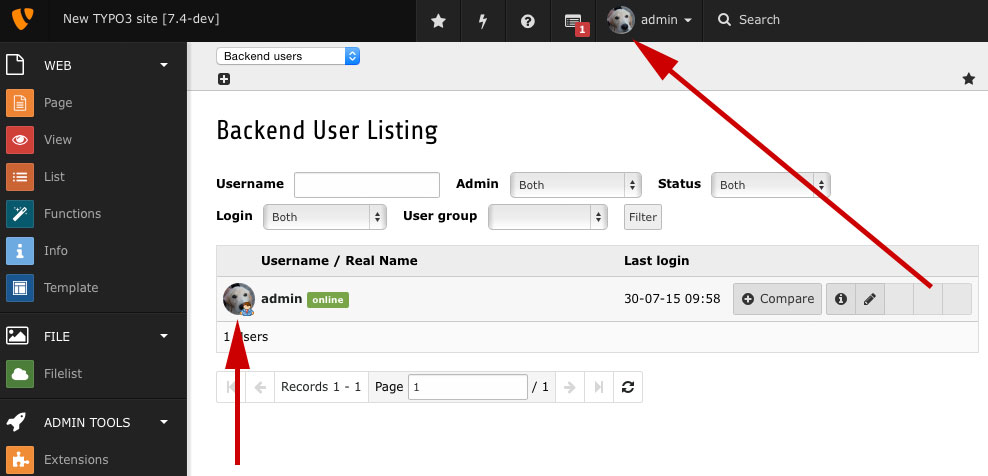
\includegraphics[width=0.7\linewidth]{BackendUserInterface/48947.jpg}
	\end{figure}

\end{frame}

% ------------------------------------------------------------------------------
% LTXE-SLIDE-START
% LTXE-SLIDE-UID:		926772f1-9743b8aa-e3a365e9-3917a610
% LTXE-SLIDE-ORIGIN:	89f348c8-db045eff-5dfc4f42-da1a2cfa English
% LTXE-SLIDE-ORIGIN:	b0f7e15a-7cc72aaa-79738ec7-643c5cec German
% LTXE-SLIDE-TITLE:		Feature: #56133 - Replace file feature for fal file list
% LTXE-SLIDE-REFERENCE:	Feature-56133-ReplaceFileFeatureForFalFileList.rst
% ------------------------------------------------------------------------------
\begin{frame}[fragile]
	\frametitle{Interface Utilisateur Backend}
	\framesubtitle{Remplacement de fichiers}

	Les fichiers de la liste des enregistrements FAL peuvent être \textbf{remplacés} (nécessite
	l'activation de la «~vue étendue~»).
	Le nom du fichier peut être gardé ou mis à jour.

	\begin{figure}
		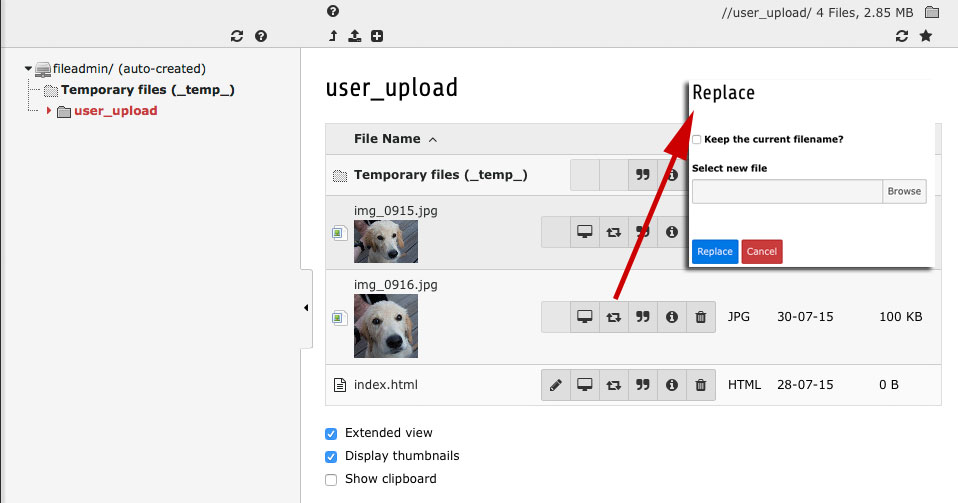
\includegraphics[width=0.75\linewidth]{BackendUserInterface/56133.jpg}
	\end{figure}

\end{frame}

% ------------------------------------------------------------------------------
% LTXE-SLIDE-START
% LTXE-SLIDE-UID:		ccf7474f-cc4adcc6-942caeb1-5ff94074
% LTXE-SLIDE-ORIGIN:	7e5987f7-9a91ea61-8564c721-0f8d5e4a English
% LTXE-SLIDE-ORIGIN:	613354cc-9475feef-bec620c5-31170549 German
% LTXE-SLIDE-TITLE:		Feature: #67574 - Display online status in backend user list
% LTXE-SLIDE-REFERENCE:	Feature-67574-DisplayOnlineStatusInBackendUserList.rst
% ------------------------------------------------------------------------------
\begin{frame}[fragile]
	\frametitle{Interface Utilisateur Backend}
	\framesubtitle{Affichage de l'état connecté des utilisateurs}

	L'état de connexion des utilisateurs backend est affiché dans le module «~Utilisateurs Backend~».

	\begin{figure}
		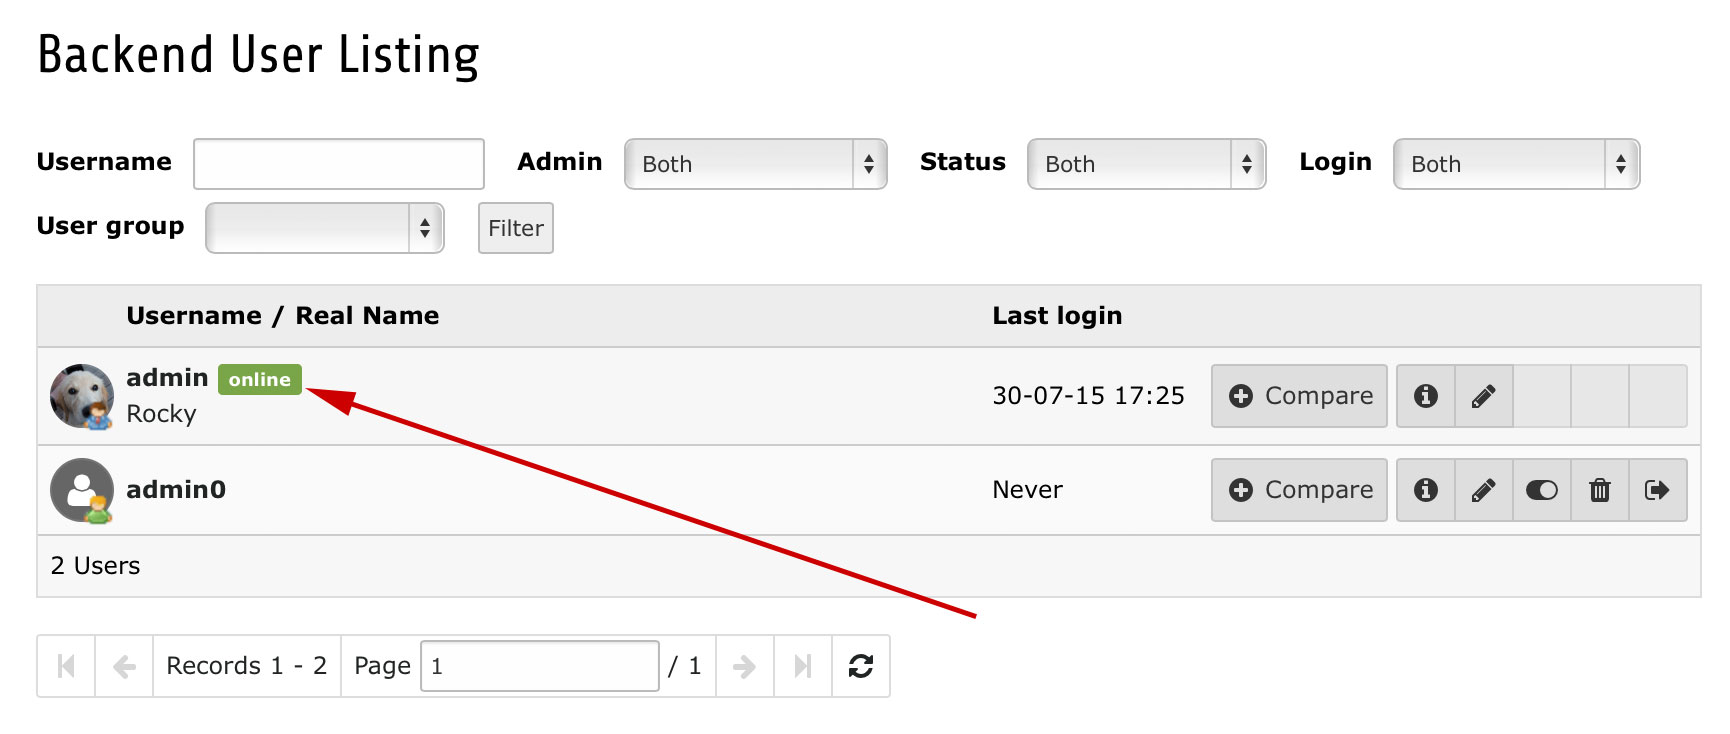
\includegraphics[width=0.9\linewidth]{BackendUserInterface/67574.jpg}
	\end{figure}

\end{frame}

% ------------------------------------------------------------------------------
% LTXE-SLIDE-START
% LTXE-SLIDE-UID:		002cd0d2-f4f85207-b164e9b9-69f5e7fc
% LTXE-SLIDE-ORIGIN:	0154fc51-74683590-ebbe8559-ce6a0d57 English
% LTXE-SLIDE-ORIGIN:	00c93fe2-9d128591-20b71814-13556f43 German
% LTXE-SLIDE-TITLE:		FormEngine: Drop "Show secondary options"
% LTXE-SLIDE-REFERENCE:	https://forge.typo3.org/issues/67753
% ------------------------------------------------------------------------------
\begin{frame}[fragile]
	\frametitle{Interface Utilisateur Backend}
	\framesubtitle{«~Options secondaires~» retiré}

	La case à cocher «~Afficher les options secondaires (palettes)~», l'option TSconfig de page
	\texttt{options.enableShowPalettes} et les configurations TCA sont retirées. Les palettes sont
	toujours visibles et ne peuvent plus être masquées.

	\begin{figure}
		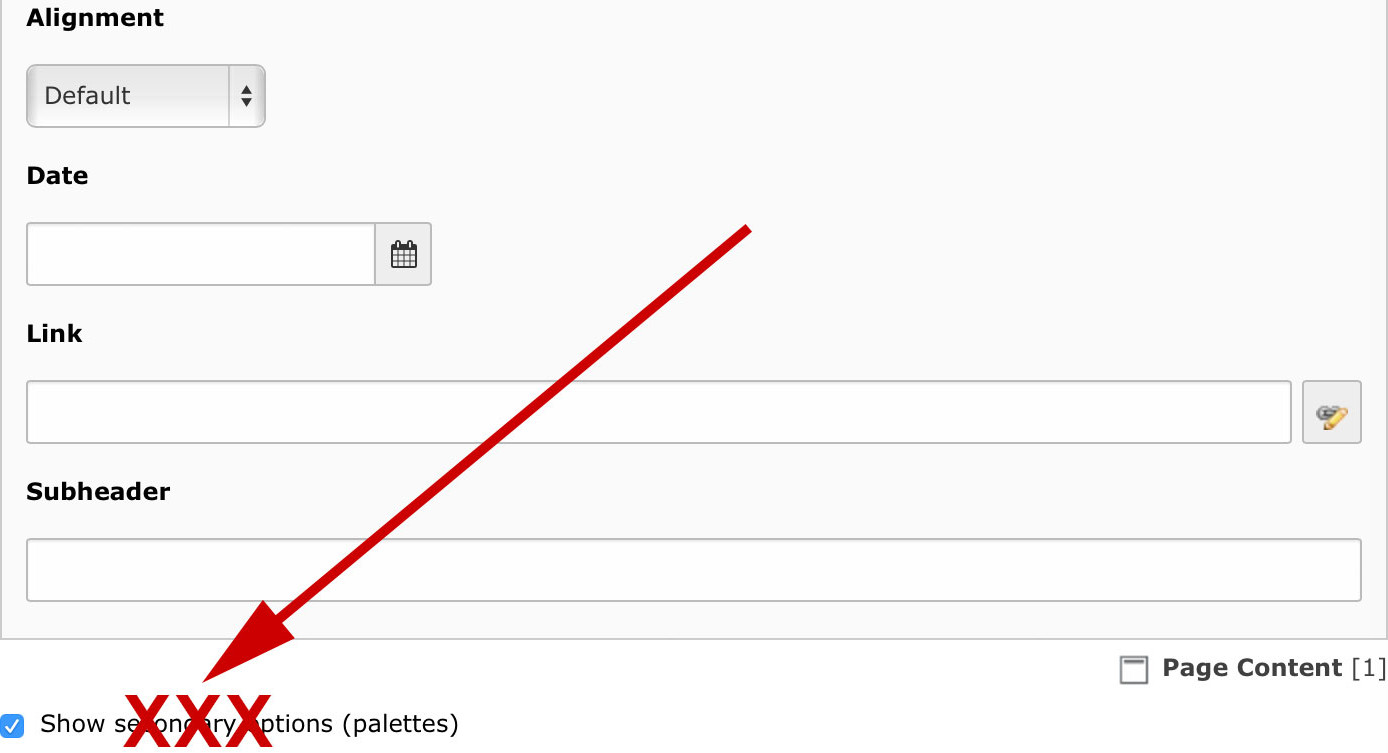
\includegraphics[width=0.6\linewidth]{BackendUserInterface/67753.jpg}
	\end{figure}

\end{frame}

% ------------------------------------------------------------------------------
% LTXE-SLIDE-START
% LTXE-SLIDE-UID:		cf10c2d8-7243609b-8d27e897-5dc8cc29
% LTXE-SLIDE-ORIGIN:	f9b24e36-28e8872c-41297de9-52467554 English
% LTXE-SLIDE-ORIGIN:	bab4e93d-0a6d4612-41b2f67e-47c37ff7 German
% LTXE-SLIDE-TITLE:		Feature: #67578 - Add description-field for backend-users
% LTXE-SLIDE-REFERENCE:	Feature-67578-AddDescriptionFieldForBeUsers.rst
% ------------------------------------------------------------------------------
\begin{frame}[fragile]
	\frametitle{Interface Utilisateur Backend}
	\framesubtitle{Description pour les Utilisateurs Backend}

	Le nouveau champ «~Description~» est ajouté aux enregistrements d'utilisateur backend.

	\begin{figure}
		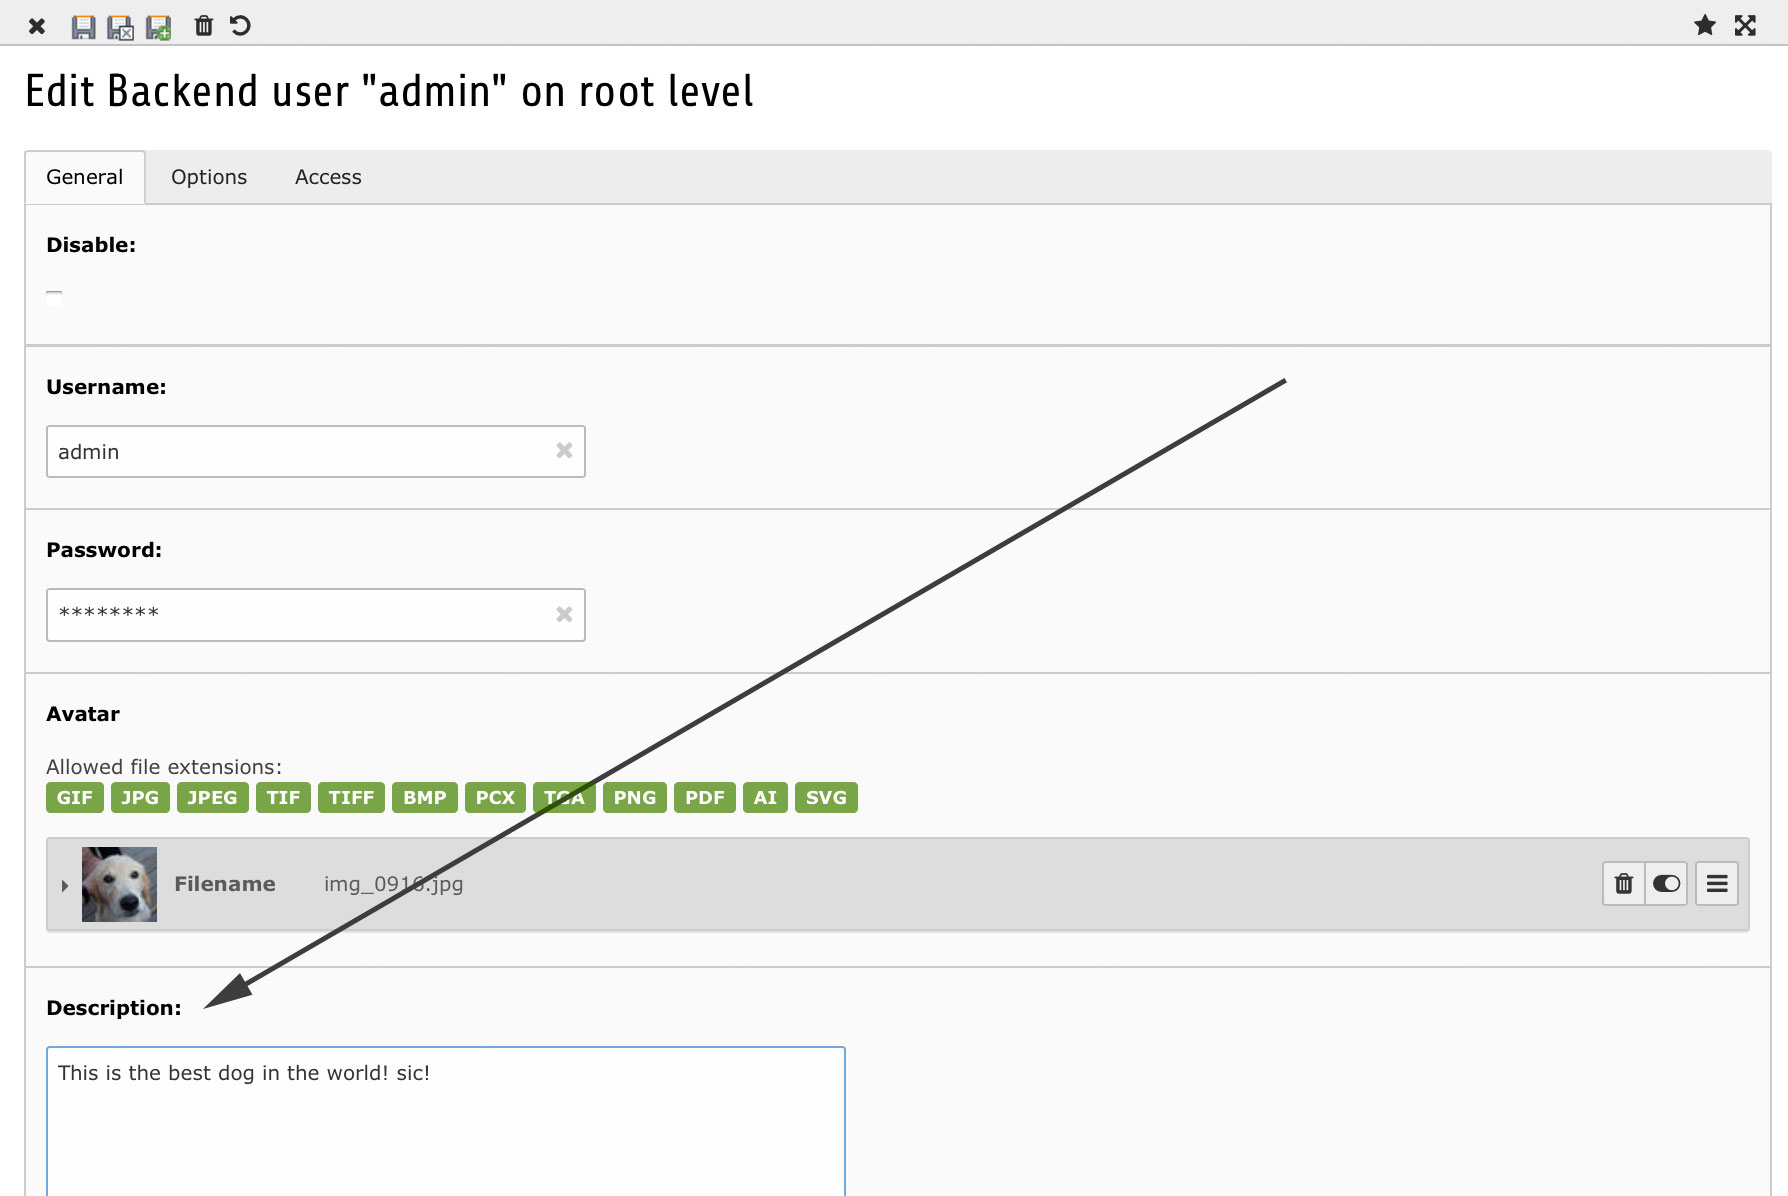
\includegraphics[width=0.65\linewidth]{BackendUserInterface/67578.jpg}
	\end{figure}

\end{frame}

% ------------------------------------------------------------------------------
% LTXE-SLIDE-START
% LTXE-SLIDE-UID:		0d7bbc76-8b4855a3-e6955eae-7fbd7872
% LTXE-SLIDE-ORIGIN:	83db5442-fa2edfcc-925dd5b6-4afe26f5 English
% LTXE-SLIDE-ORIGIN:	649bd9ee-240381c8-950424ea-f032775b German
% LTXE-SLIDE-TITLE:		Feature: #67603 - Introduce TCA > ctrl > descriptionColumn
% LTXE-SLIDE-REFERENCE:	Feature-67603-IntroduceTcaDescriptionColumn.rst
% ------------------------------------------------------------------------------
\begin{frame}[fragile]
	\frametitle{Interface Utilisateur Backend}
	\framesubtitle{Colonne Description}

	En configurant une colonne (habituellement \texttt{description}) dans la configuration TCA
	\texttt{['TCA']['ctrl']['descriptionColumn']}, une description peut être affichée
	(améliore l'usabilité pour les éditeurs et administrateurs).

	\begin{figure}
		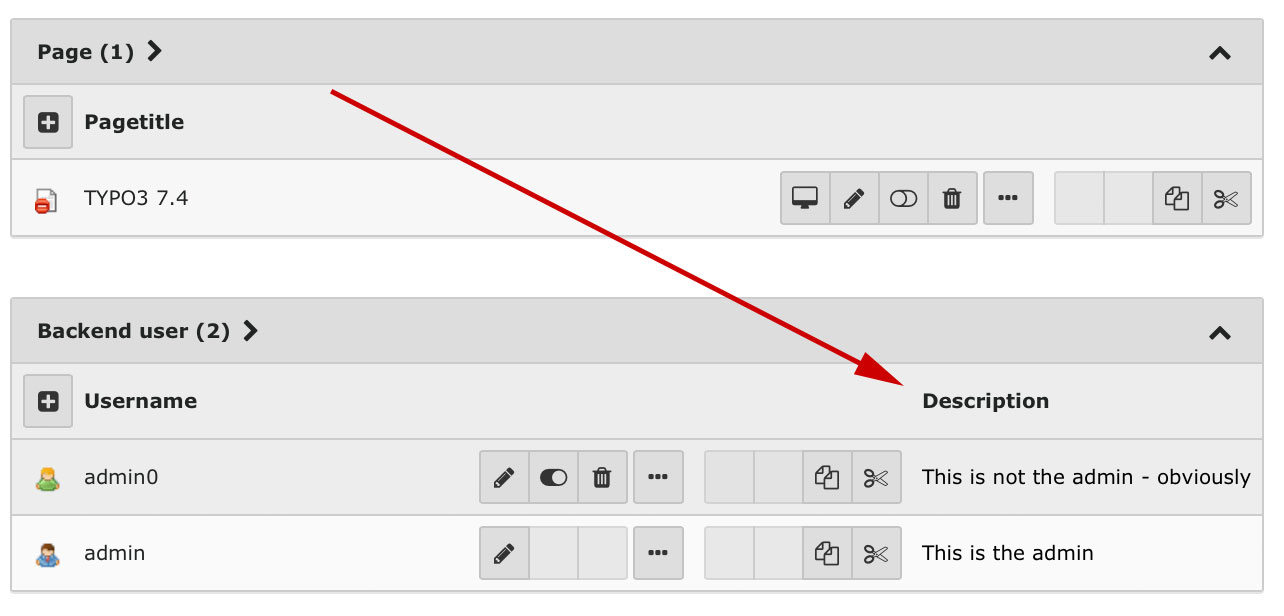
\includegraphics[width=0.7\linewidth]{BackendUserInterface/67603.jpg}
	\end{figure}

\end{frame}

% ------------------------------------------------------------------------------
% LTXE-SLIDE-START
% LTXE-SLIDE-UID:		7bc2676c-bc154957-bd65d950-a0e99254
% LTXE-SLIDE-ORIGIN:	7c5400a9-c4b667f3-1a0c046a-9dd3b6a9 English
% LTXE-SLIDE-ORIGIN:	2eeaec46-1929743b-8e6f9285-13d20d3c German
% LTXE-SLIDE-TITLE:		Feature: #59570 - Add description-field for filemounts
% LTXE-SLIDE-REFERENCE:	Feature-59570-AddDescriptionFieldForFilemounts.rst
% ------------------------------------------------------------------------------
\begin{frame}[fragile]
	\frametitle{Interface Utilisateur Backend}
	\framesubtitle{Description pour les montages de fichiers}

	Le nouveau champ «~Description~» est ajouté aux enregistrements points de montage de fichiers.
	Le champ permet de renseigner une courte description indiquant l'utilité du point de montage, quels
	documents il peut contenir, etc.

	\begin{figure}
		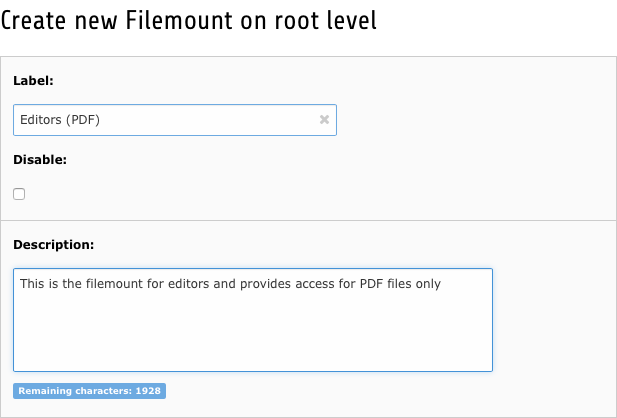
\includegraphics[width=0.5\linewidth]{BackendUserInterface/59570.png}
	\end{figure}

\end{frame}

% ------------------------------------------------------------------------------
% LTXE-SLIDE-START
% LTXE-SLIDE-UID:		69769248-1af98c22-4013c693-848acf38
% LTXE-SLIDE-ORIGIN:	d00f63c4-05272792-21a0a301-4d6a726c English
% LTXE-SLIDE-ORIGIN:	879b1dda-9167d830-373f7457-0391ebee German
% LTXE-SLIDE-TITLE:		Feature: #68197 - Show a dialog for existing files on upload
% LTXE-SLIDE-REFERENCE:	Feature-68197-ShowADialogForExistingFilesOnUpload.rst
% ------------------------------------------------------------------------------
\begin{frame}[fragile]
	\frametitle{Interface Utilisateur Backend}
	\framesubtitle{Confirmation de l'écrasement des fichiers}

	Si un fichier envoyé écrase un fichier existant, une fenêtre de confirmation est affichée,
	permettant à l'utilisateur de choisir une action (i.e. remplacer, renommer ou ignorer).

	\begin{figure}
		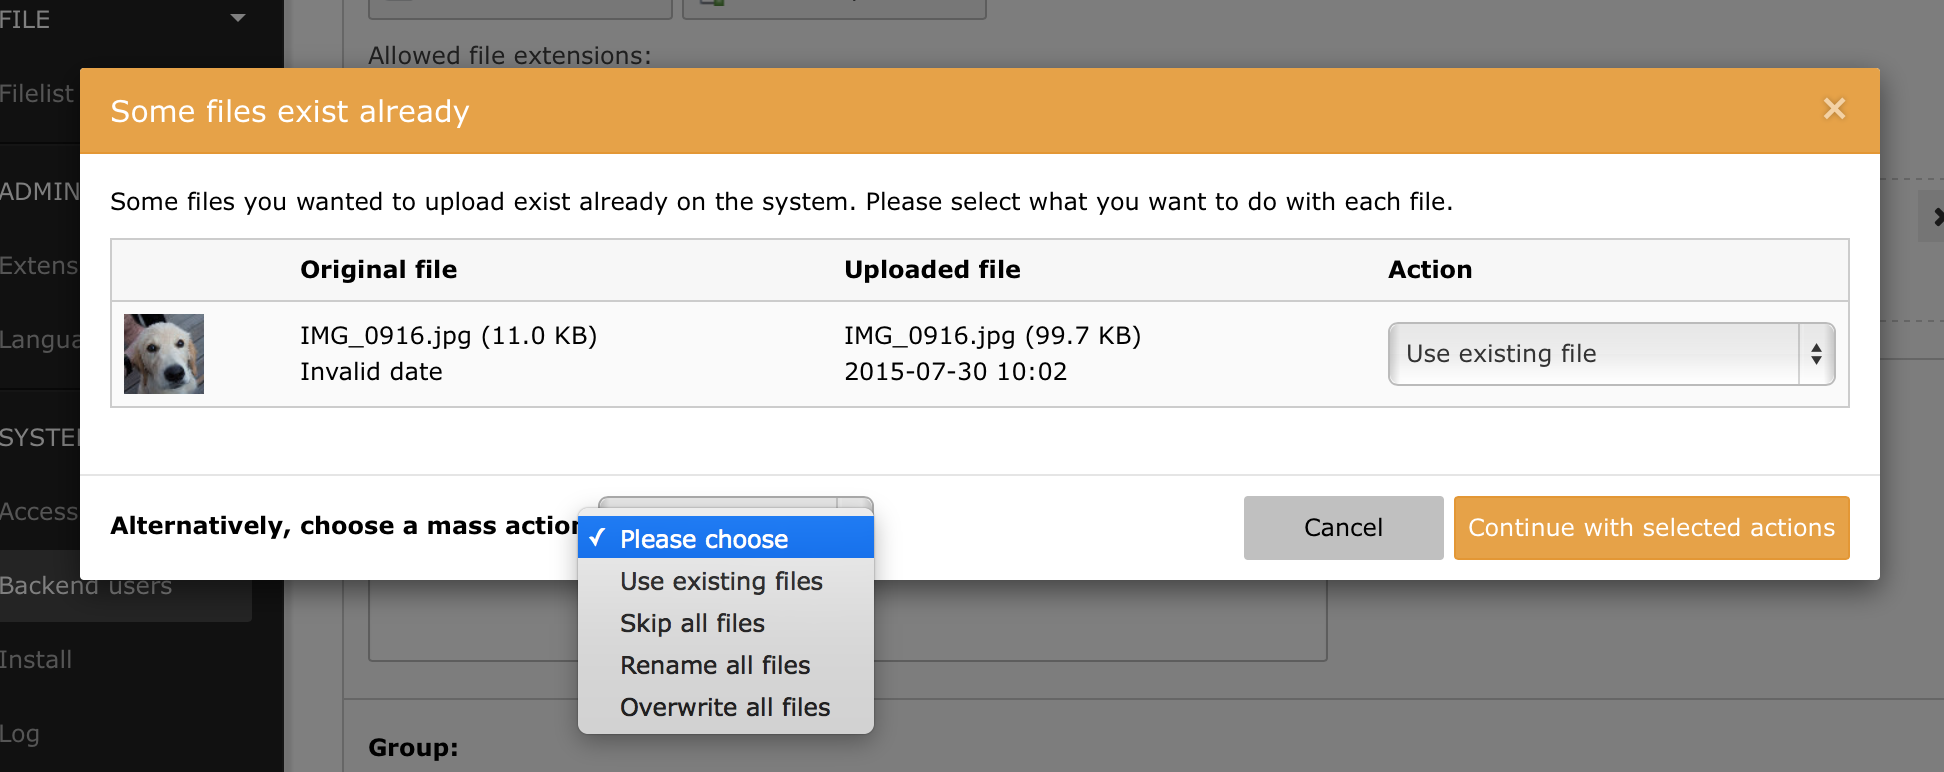
\includegraphics[width=0.9\linewidth]{BackendUserInterface/68197.png}
	\end{figure}

\end{frame}


% ------------------------------------------------------------------------------
% LTXE-SLIDE-START
% LTXE-SLIDE-UID:		21ad979c-1f68a1aa-9218f050-f4225719
% LTXE-SLIDE-ORIGIN:	31d7dd8e-a3c71be4-309850ab-45a7db72 English
% LTXE-SLIDE-ORIGIN:	f4baa7b8-2237ad1d-5c4be365-a845f207 German
% LTXE-SLIDE-TITLE:		Feature: #68218 - Lock edit for tt_content
% LTXE-SLIDE-REFERENCE:	Feature-68218-LockEditForTt_content.rst
% ------------------------------------------------------------------------------
\begin{frame}[fragile]
	\frametitle{Interface Utilisateur Backend}
	\framesubtitle{Restriction d'édition des contenus}

	Les éléments de contenu peuvent être restreints à l'édition aux administrateurs uniquement
	(similaire à la fonction «~Restreindre à l'édition par les non-admins~» des pages).

	\begin{figure}
		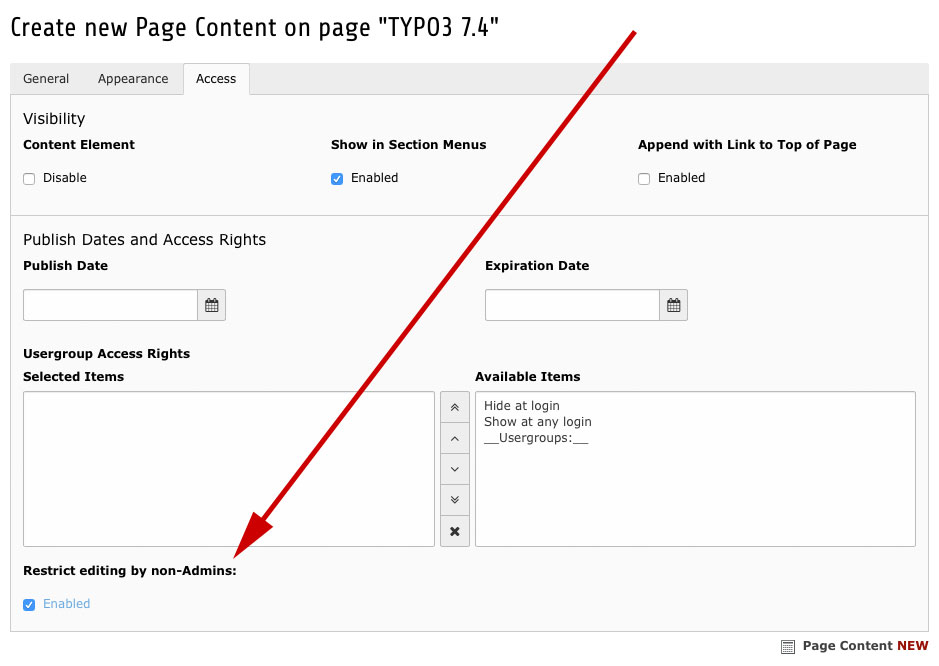
\includegraphics[width=0.55\linewidth]{BackendUserInterface/68218.jpg}
	\end{figure}

\end{frame}

% ------------------------------------------------------------------------------
% LTXE-SLIDE-START
% LTXE-SLIDE-UID:		af4dee23-c926d7fb-d334b311-d431c50e
% LTXE-SLIDE-ORIGIN:	4e60055a-266e3e24-7baa1613-1226575e English
% LTXE-SLIDE-ORIGIN:	bc83e40f-9b7bac03-ea5f07c4-be27eb56 German
% LTXE-SLIDE-TITLE:		Feature: #68315 - Include pageTSconfig file (1)
% LTXE-SLIDE-REFERENCE:	Feature-68315-IncludeAPageTSconfigFileInPagePropertiesLikeTSStaticTemplates.rst
% ------------------------------------------------------------------------------
\begin{frame}[fragile]
	\frametitle{Interface Utilisateur Backend}
	\framesubtitle{Inclusion de fichiers TSconfig statiques (1)}

	Dans les propriétés des pages, une option permet d'inclure des fichiers de TSconfig de page
	(de la même manière que pour les gabarits TypoScript).

	\begin{figure}
		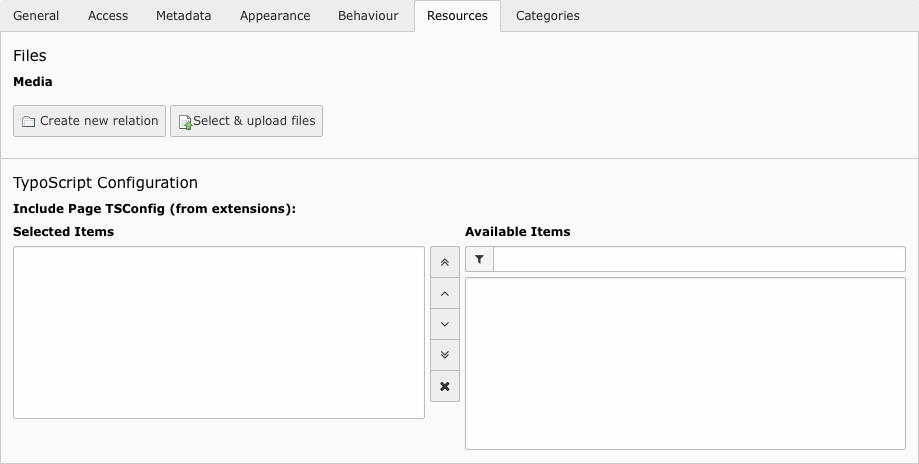
\includegraphics[width=0.8\linewidth]{BackendUserInterface/68315.png}
	\end{figure}

\end{frame}

% ------------------------------------------------------------------------------
% LTXE-SLIDE-START
% LTXE-SLIDE-UID:		85703c83-b86dfbba-9978b536-17bc6606
% LTXE-SLIDE-ORIGIN:	4f5cb411-3ea84dfd-84edb16d-433b9fc5 English
% LTXE-SLIDE-ORIGIN:	9b7bac03-ea5f07c4-be27eb56-ac03e27e German
% LTXE-SLIDE-TITLE:		Feature: #68315 - Include pageTSconfig file (2)
% LTXE-SLIDE-REFERENCE:	Feature-68315-IncludeAPageTSconfigFileInPagePropertiesLikeTSStaticTemplates.rst
% ------------------------------------------------------------------------------
\begin{frame}[fragile]
	\frametitle{Interface Utilisateur Backend}
	\framesubtitle{Inclusion de fichiers TSconfig statiques (2)}

	% decrease font size for code listing
	\lstset{basicstyle=\tiny\ttfamily}

	La méthode suivante inscrit un fichier TSconfig de page~:

	\begin{lstlisting}
		\TYPO3\CMS\Core\Utility\ExtensionManagementUtility::registerPageTSConfigFile(
		  'extension_name',
		  'Configuration/PageTS/myPageTSconfigFile.txt',
		  'My special configuration'
		);
	\end{lstlisting}

\end{frame}

% ------------------------------------------------------------------------------
% LTXE-SLIDE-START
% LTXE-SLIDE-UID:		79a0e595-181e6c6f-9afd1f7e-cc13c5dd
% LTXE-SLIDE-ORIGIN:	c00b2bfd-2c1b02b0-a7ef9cd0-62f147d2 English
% LTXE-SLIDE-ORIGIN:	f8d888b1-b93dcf4a-e20b976e-9a5c277e German
% LTXE-SLIDE-TITLE:		Feature: #68395 - Allow real copies of content elements into foreign languages
% LTXE-SLIDE-REFERENCE:	Feature-68395-AllowRealCopiesOfContentElementsIntoForeignLanguages.rst
% ------------------------------------------------------------------------------
\begin{frame}[fragile]
	\frametitle{Interface Utilisateur Backend}
	\framesubtitle{Réelle copie des contenus}

	Un nouveau bouton est ajouté pour toutes les colonnes du module «~Page~» permettant de copier
	\textit{réellement} les contenus dans une langue (pas seulement des références).

	\begin{figure}
		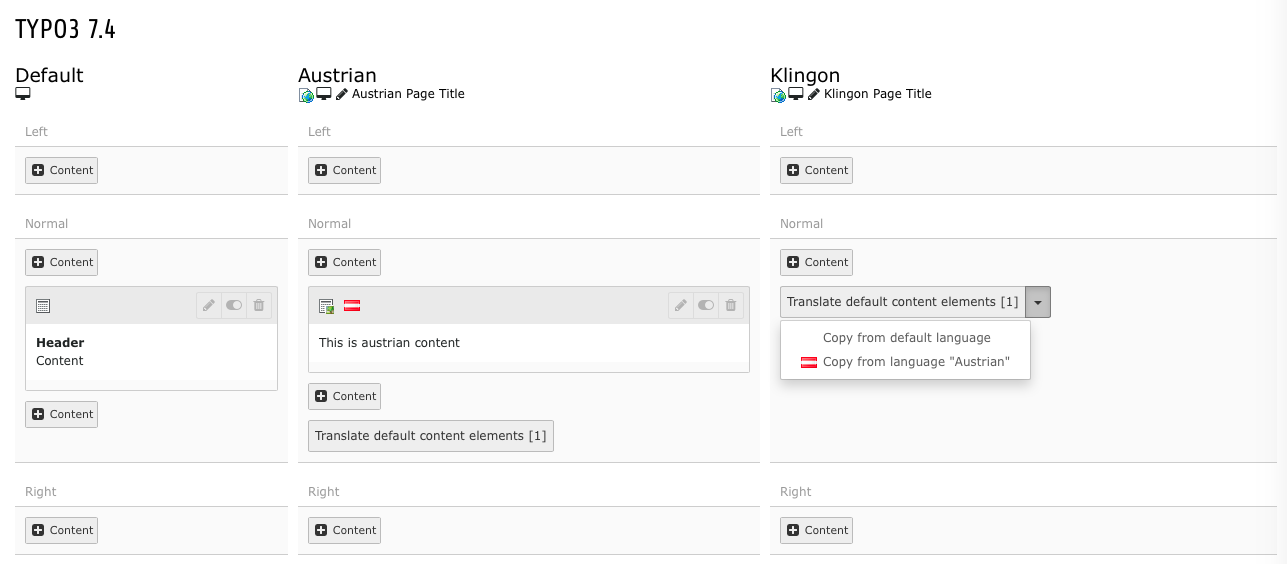
\includegraphics[width=0.9\linewidth]{BackendUserInterface/68395.png}
	\end{figure}

\end{frame}


